\documentclass[tikz,border=10pt]{standalone}
\usepackage[T1]{fontenc}
\usepackage{helvet}
\renewcommand{\familydefault}{\sfdefault}
\usepackage{tikz}
\usetikzlibrary{arrows.meta,positioning,shapes.multipart,shapes.geometric,fit,backgrounds,calc,shadows}

\definecolor{navy}{HTML}{1F3A5F}
\definecolor{teal}{HTML}{0C6B58}
\definecolor{amber}{HTML}{D9822B}
\definecolor{crimson}{HTML}{B42318}
\definecolor{violet}{HTML}{6B21A8}
\definecolor{sky}{HTML}{2186EB}
\definecolor{slate}{HTML}{486581}
\definecolor{mist}{HTML}{F0F4F8}
\definecolor{line}{HTML}{9FB3C8}

\tikzset{
  >={Stealth[length=2.6mm]},
  box/.style={draw=navy, very thick, rounded corners=3pt, fill=white, align=center,
    inner sep=5pt, font=\small, minimum height=9mm},
  softbox/.style={box, draw=slate, thick, fill=mist},
  layer/.style={draw=line, dashed, rounded corners=6pt, inner sep=7pt},
  layertitle/.style={font=\bfseries\small, text=slate, anchor=north west},
  flow/.style={->, thick, draw=navy},
  dflow/.style={->, thick, draw=slate, dashed},
  lbl/.style={font=\scriptsize, text=slate, fill=white, inner sep=1.5pt},
  umlclass/.style={draw=navy, thick, fill=white, rectangle split, rectangle split parts=3,
    rectangle split part fill={navy!12,white,white}, align=left, font=\scriptsize,
    inner sep=3pt, text width=#1},
  umlclass/.default=38mm,
}

\tikzset{
  ext/.style={draw=navy, very thick, fill=mist, minimum width=3.4cm, minimum height=1.3cm,
    align=center, font=\small\bfseries},
  proc/.style={circle, draw=teal, very thick, fill=white, align=center, font=\small,
    minimum size=4.2cm},
  df/.style={->, thick, draw=navy},
  dl/.style={font=\scriptsize, fill=white, align=center, inner sep=2pt},
}
\begin{document}
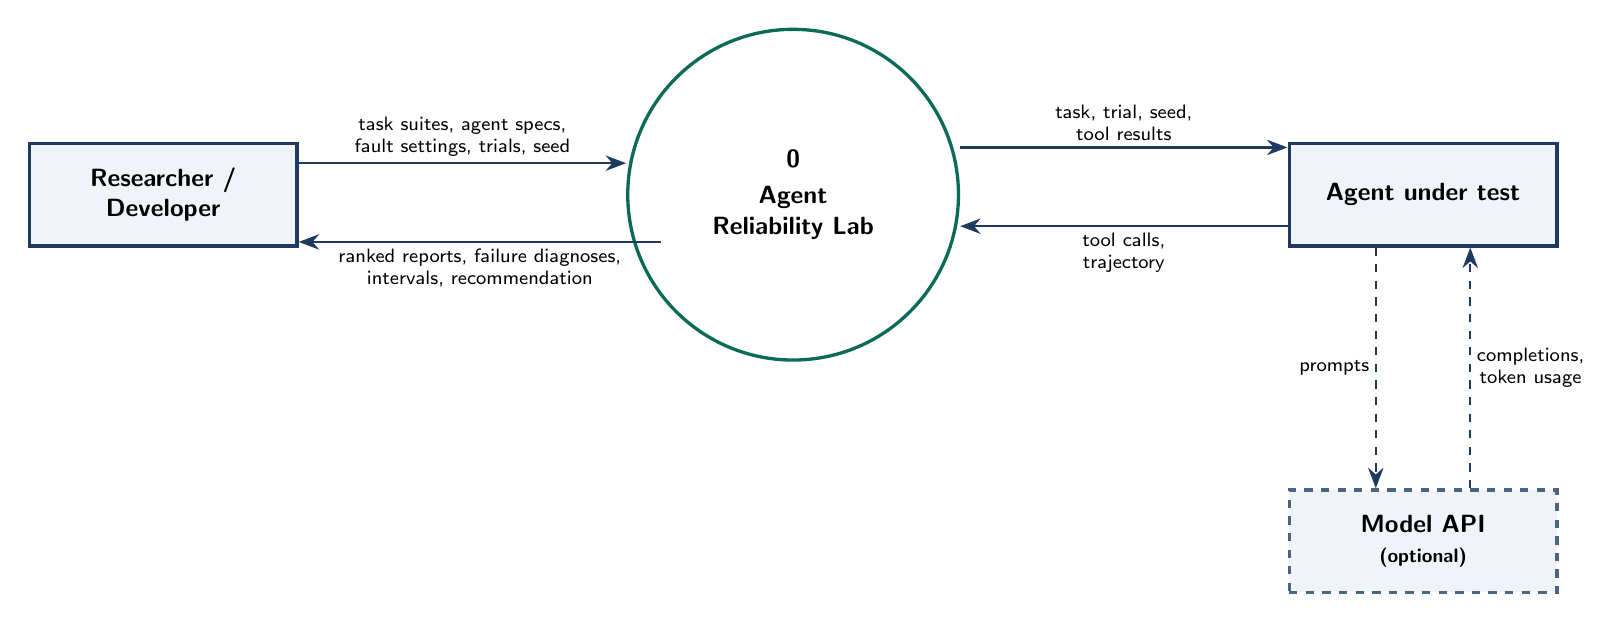
\begin{tikzpicture}[x=1cm,y=1cm]
  \node[proc] (lab) at (0,0) {\textbf{0}\\[2pt]\textbf{Agent}\\\textbf{Reliability Lab}};
  \node[ext] (user) at (-8,0) {Researcher /\\Developer};
  \node[ext] (agent) at (8,0) {Agent under test};
  \node[ext, draw=slate, dashed] (model) at (8,-4.4) {Model API\\\scriptsize (optional)};

  \draw[df] ([yshift=4mm]user.east) -- node[dl, above] {task suites, agent specs,\\fault settings, trials, seed} ([yshift=4mm]user.east -| lab.west);
  \draw[df] ([yshift=-6mm]lab.west -| user.east) ++(4.6,0) -- node[dl, below] {ranked reports, failure diagnoses,\\intervals, recommendation} ([yshift=-6mm]user.east);
  \draw[df] ([yshift=6mm]lab.east) -- node[dl, above] {task, trial, seed,\\tool results} ([yshift=6mm]agent.west);
  \draw[df] ([yshift=-4mm]agent.west) -- node[dl, below] {tool calls,\\trajectory} ([yshift=-4mm]lab.east);
  \draw[df, dashed] ([xshift=-6mm]agent.south) -- node[dl, left] {prompts} ([xshift=-6mm]model.north);
  \draw[df, dashed] ([xshift=6mm]model.north) -- node[dl, right] {completions,\\token usage} ([xshift=6mm]agent.south);
\end{tikzpicture}
\end{document}
